\documentclass[11pt, a4paper]{article}

\usepackage[left=3cm, right=3cm, top=3cm, bottom=3cm]{geometry}
\usepackage{graphicx}


\title{Monte Carlo Methods - Sheet 1}
\author{Tobias Sizmann}

\begin{document}
\maketitle
\section{Exercise 2 - Expectation values and standard error}
    \subsection{Distribution of expectation values}
        \begin{figure}
            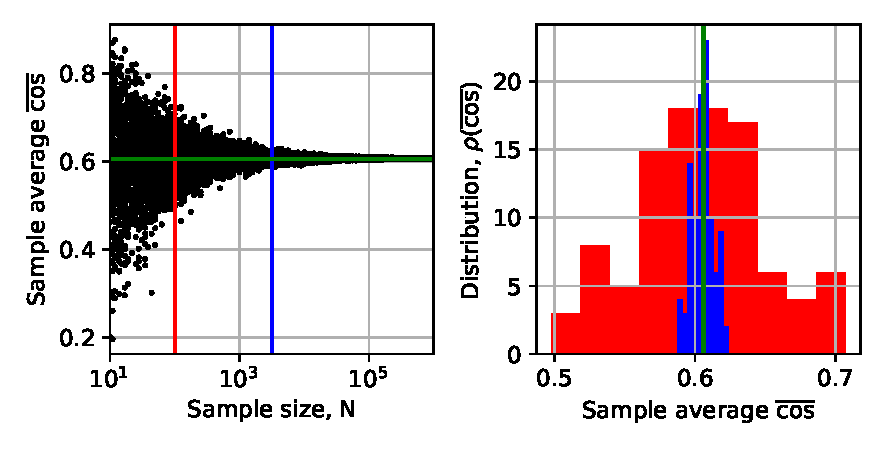
\includegraphics{fig1.pdf}
            \label{fig1}
            \caption{\textbf{Behaviour of sample means in respect to the sample size:} a) 100 samples were generated (normal distribution with $\mu = 0, \sigma = 1$) for each different sample sizes N from $10$ to $10^6$ and the resulting means $\bar{f} = \overline{\cos}$ were plotted in black. A logarithmic scale was choosen for N. The green line marks the expectation value $\langle \cos \rangle_p$. The red line and blue lines mark the values $N = 10^2$ and $N = 3162 \approx 10^{3.5}$, respectively. b) The red and blue cross sections from plot a) are plotted as histograms. They roughly follow a normal distribution around the expectation value $\langle \cos \rangle$ marked by the green line.}
        \end{figure}

        Consider a normal probability distribution $p = \mathcal{N}(\mu = 0, \sigma = 1)$ and the measurement $f(x) = \cos(x)$ defined on configurations $x$ following this distribution. We want to investigate how the means $\bar{f}$ of samples $S_N$ with sample size $N$ behave. To this end we consider 101 values of $N$ evenly distributed from $10$ to $10^6$. For each value $N$ we generate 100 samples with size $N$, respectively. The mean of $f(x) = \cos(x)$ is computed and analyzed. The results are depicted in fig. \ref{fig1}. In plot a) one can see that with increasing sample size the deviation decreases and the sample means converge towards the expectation value. This effect is quantitatively discussed later. In plot b) two histograms for the distributions of means $\bar{f}$ for $N = 100$ (red) and $N = 3126$ (green) are depicted. They roughly follow a gaussian distribution centered around the expectation value $\langle \cos \rangle_p \approx 0.606$. This can be seen as an experimental proof of the central limit theorem.
    \subsection{Standard error}
        \begin{figure}
            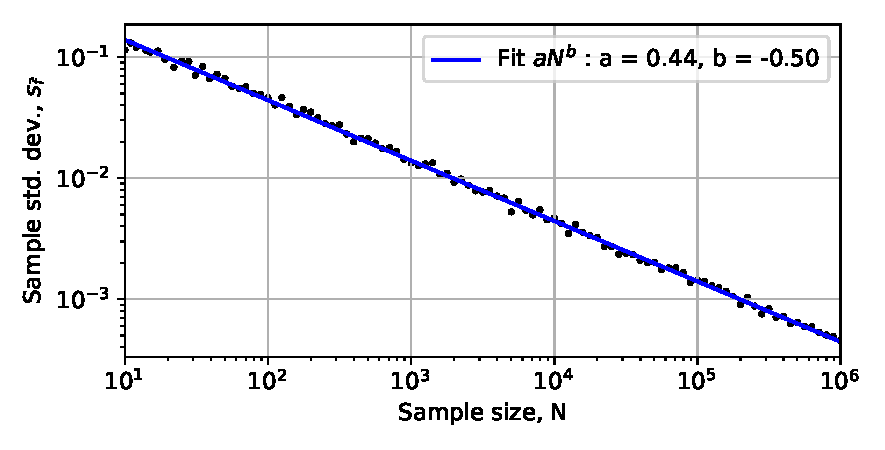
\includegraphics{fig2.pdf}
            \label{fig2}
            \caption{\textbf{Dependence of the standard error on the sample size:} a) For each N the standard deviation $\sigma_\bar{f}$ of the 100 sample means has been calculated and plotted over N. A function $aN^b$ has been fitted.}
        \end{figure}
        We now want to investigate how the standard error $\sigma_\bar{f}$ of the sample mean depends on the standard deviation $\sigma_f$ and the sample size $N$. To this end the standard deviation over 100 samples for each N has been calculated and is depicted in fig. \ref{fig2}. The central limit theorem suggests that for uncorrelated configurations the standard error behaves like $\sigma_{\bar{f}} = \frac{\sigma_f}{\sqrt{N}}$. To test this quantitatively a fit $aN^b$ has been done which returns $a = 0.44$ and $b = -0.50$. The value for $b$ perfectly coincides with the theoretical expectation. The fit parameter $a$ relates to $\sigma_f$ according to the central limit theorem. $\sigma_f$ has been calculated numerically on a sample with size $N = 10^7$ yielding a value of $\sigma_f = 0.447$ which coincides with the fit. One can conclude that the central limit theorem holds.
\end{document}
